\chapter{Contexte}
\section{Aboard Engineering}
\subsection{L'entreprise}
Aboard Engineering est un bureau d'études en automatique, électronique et informatique industrielle. Composé d'experts en contrôle et instrumentation de systèmes embarqués temps réel, ses ingénieurs développent des solutions pour des applications civiles et militaires. De la R\&D à la série, Aboard Engineering travail dans le domaine des transports (automobile, aéronotique, marin), de l'off-road (agriculture, engins de chantier, ...) et de l'industrie. Les figures \ref{fig:domaines} et  \ref{fig:metiers} sont tirées du site web d'Aboard Engineering et récapitulent les domaines et métiers de la société.

\begin{figure}[h]
	\center
	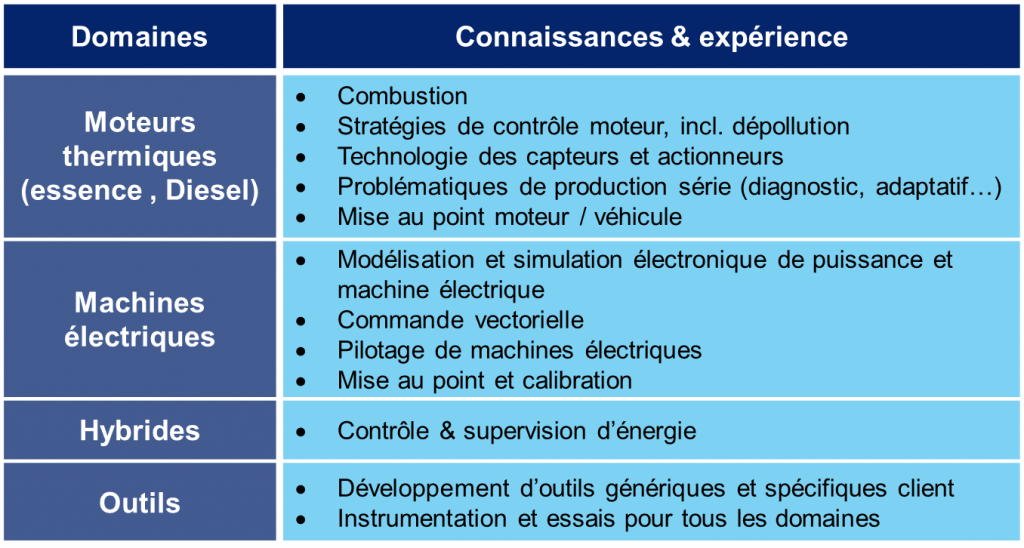
\includegraphics[scale=0.4]{images/domaines}
	\caption{Domaines -- Source : Abord Engineering}
	\label{fig:domaines}
\end{figure}

\begin{figure}[h]
	\center
	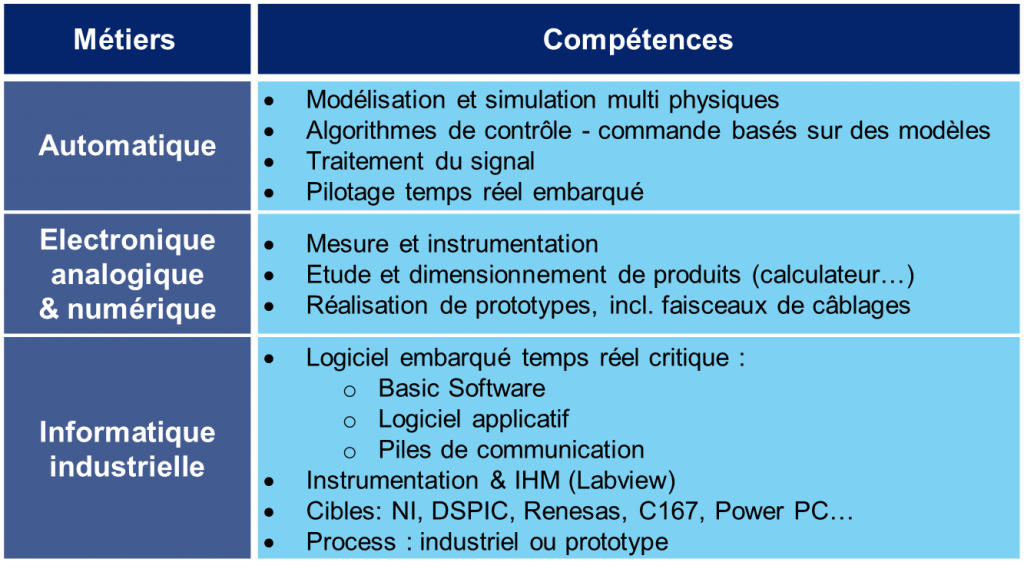
\includegraphics[scale=0.4]{images/metiers}
	\caption{Métiers et Compétences -- Source : Abord Engineering}
	\label{fig:metiers}
\end{figure}

\section{La plateforme Orianne}
\label{sec:orianne}

Aboard Engineering fournie différents types de produits et services. Je ne vais ici développer que le cas de la plateforme Orianne sur laquelle j'ai travaillé.

Orianne est un acronyme

\section{L'environnement de travail}
\lipsum
